\documentclass[aspectratio=169,sn-mathphys-num,spanish]{beamer}

\usepackage{fontspec}
\usepackage{unicode-math}
\usepackage{graphicx}
\usepackage[dvipsnames]{xcolor}
\usepackage[sorting=none]{biblatex}
\usepackage[spanish]{babel}
\usepackage{ragged2e}
\addbibresource{../document/references.bib}

\usetheme[numbering=counter, progressbar=frametitle, background=light]{metropolis}

\usecolortheme{dove}
\definecolor{primary}{RGB}{88, 24, 69}
\definecolor{secondary}{RGB}{0, 168, 150}

\setbeamercovered{transparent}
\setbeamercolor{frametitle}{fg=white, bg=primary}
\setbeamercolor{progress bar}{fg=secondary}
\setbeamerfont{frametitle}{size=\large, series=\bfseries}
\setbeamerfont{title}{size=\LARGE, series=\bfseries}
\setbeamercolor{alerted text}{fg=secondary}
\setbeamercolor{block title}{fg=primary}
\setbeamercolor{block body}{bg=white}

\title{Radiotelescopios de bajo costo para la enseñanza de la Radioastronomía en Colegios}
\author{Laura Herrera \and Bryan Martinez \and Julian Avila}
\institute{Universidad Distrital Francisco José de Caldas}
\date{\today}

\begin{document}

\begin{frame}
	\titlepage
\end{frame}

\begin{frame}{Outline}
	\setbeamertemplate{section in toc}[circle]
	\tableofcontents
\end{frame}

\section{Problemática}
La educación en ciencias y tecnología en las instituciones públicas de Bogotá
enfrenta grandes desafíos, entre ellos la falta de infraestructura
especializada que permita a los estudiantes acceder a experiencias prácticas en
el campo de la astronomía.
A pesar del creciente interés por la exploración del universo y el desarrollo de
la tecnología aeroespacial, la enseñanza en estos campos sigue siendo teórica y
limitada en recursos que permitan la experimentación directa.

Actualmente, los programas de educación secundaria en ciencias naturales y
física abordan temáticas relacionadas con la astronomía de manera superficial,
sin contar con herramientas que faciliten la observación y el análisis de datos
astronómicos reales.
Esto genera una brecha de acceso al conocimiento y una disminución del interés
de los estudiantes por carreras en ciencia, tecnología, ingeniería y matemáticas,
lo que afecta el desarrollo científico y tecnológico del país a largo plazo.

Además, la astronomía observacional suele estar restringida a telescopios
ópticos, los cuales dependen de condiciones atmosféricas favorables y presentan
limitaciones en la exploración de otros espectros electromagnéticos.
La falta de acceso a tecnologías complementarias, como los radiotelescopios,
impide que los estudiantes puedan explorar nuevas formas de observación del
universo y desarrollar habilidades en el análisis de datos astronómicos.


\section{Proyecto}
\begin{frame}{\textbf{Propuesta del Proyecto}}
  \begin{columns}
    \column{0.55\textwidth}
    \begin{block}{\textbf{Radiotelescopios de Bajo Costo}}
      \begin{itemize}
        \item \textbf{Construcción} de radiotelescopios en instituciones públicas de Bogotá.
          \pause
        \item \textbf{Observaciones} sin depender de condiciones atmosféricas.
          \pause
        \item \textbf{Fomento} de habilidades analíticas, matemáticas y físicas.
          \pause
        \item \textbf{Impulso} a la cultura científica y tecnológica.
      \end{itemize}
    \end{block}
    \column{0.4\textwidth}
    \centering
    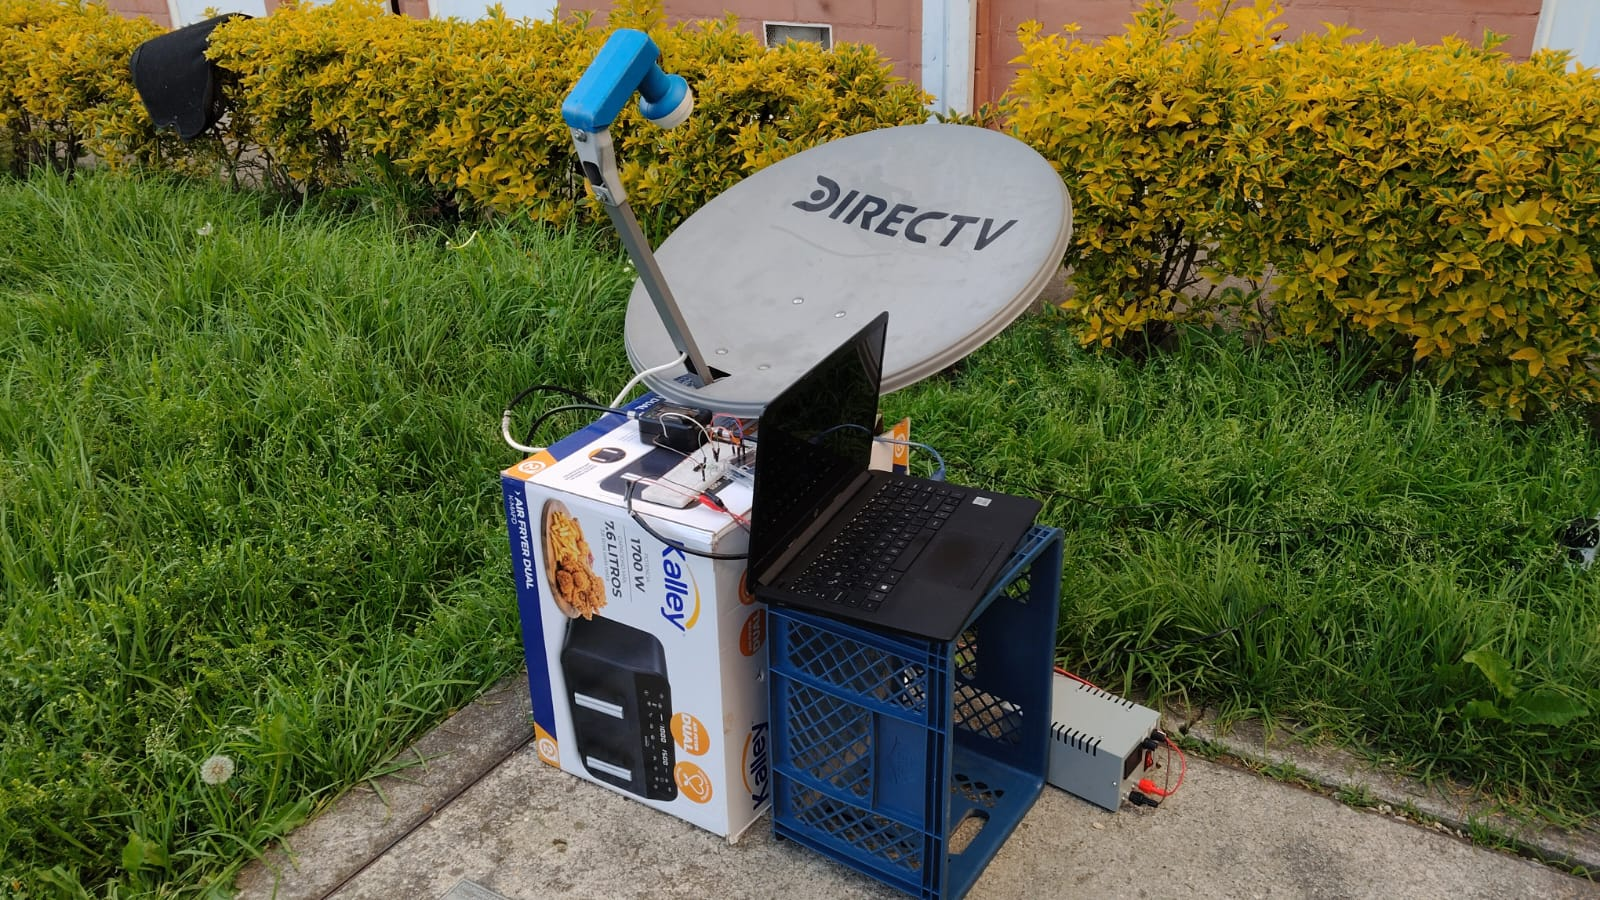
\includegraphics[width=\linewidth]{./Figures/radiotelescope.jpeg}
    \newline
    \small{\textit{Radiotelescopio didáctico de bajo costo}}
  \end{columns}
\end{frame}


\section{Objetivos}
\begin{frame}{\textbf{Objetivo General}}
  \begin{block}{}
    \centering
    \textbf{Promover} el conocimiento en \alert{ciencia y tecnología} en instituciones educativas, mediante la \alert{construcción e implementación} de radiotelescopios de bajo costo.
  \end{block}
\end{frame}

\begin{frame}{\textbf{Objetivos Específicos}}
  \begin{itemize}
    \item \textbf{Construir} radiotelescopios de \alert{bajo costo} adaptados a instituciones educativas de Bogotá.
      \pause
    \item \textbf{Analizar} la \alert{oferta y demanda} de radiotelescopios en el sector educativo.
      \pause
    \item \textbf{Seleccionar} los \alert{colegios} donde se implementará el proyecto.
      \pause
    \item \textbf{Determinar} los \alert{costos} de construcción e implementación.
  \end{itemize}
\end{frame}


\section{Metodología}
Este proyecto se enmarca dentro de una investigación aplicada, la cual busca    
generar conocimiento con un propósito práctico y concreto: la implementación de 
radiotelescopios en instituciones educativas para mejorar la enseñanza de la    
astronomía y fomentar el desarrollo de habilidades científicas en los           
estudiantes.                                                                    

En este caso, la investigación aplicada se centra en evaluar, diseñar           
e implementar una infraestructura tecnológica educativa que pueda ser utilizada 
directamente en el ámbito académico. Se utilizarán métodos cuantitativos        
y cualitativos para analizar la viabilidad del proyecto, su impacto en la       
educación y su sostenibilidad a largo plazo.                                    

Inicialmente, los radiotelescopios serán instalados en colegios privados, ya
que estas instituciones pueden colaborar con la financiación del proyecto.
Además, suelen contar con  mayor flexibilidad administrativa, lo cual facilita
la implementación inicial y la evaluación de los resultados. Esta estrategia
permitirá consolidar la infraestructura y los procesos educativos necesarios,
con miras a expandir posteriormente la iniciativa hacia los colegios públicos
de Bogotá, garantizando así un mayor alcance e inclusión educativa.

Para la implementación del proyecto de construcción de radiotelescopios en
instituciones de educación pública en Bogotá, se propone la siguiente
metodología:

\begin{itemize}

\item \textbf{Estudio de mercado de radiotelescopios de bajo costo:} Los 
radiotelescopios que se construirán son de bajo costo, es decir, se busca 
disminuir al mínimo los costos de la producción, por esto mismo, si se cuenta 
con la financiación de diferentes instituciones de educación privada, se puede 
ofrecer un radiotelescopio por institución.

Para ello, tomaremos como referencia el plan desarrollado por la Secretaría de
Educación del Distrito en alianza con el Instituto Distrital de las Artes, en
el que se incluyeron 32 colegios de 12 localidades de Bogotá, como se muestra
en la siguiente noticia:
\url{https://www.educacionbogota.edu.co/portal_institucional/noticia/la-
astronomia-llego-este-ano-21-mil-estudiantes-de-colegios-oficiales-de-bogota}

Aunque nuestra propuesta solo contempla 10 instituciones educativas
inicialmente, debido a las limitaciones presupuestales que impiden la
producción de más radiotelescopios.

\item \textbf{Estudio técnico de los materiales necesarios:} Para la 
construcción del radiotelescopio se necesita una antena parabólica, un arduino 
R3, un computador con el software correspondiente para el correcto 
funcionamiento del arduino, un buscador de satélites y un circuito amplificado, 
encargado de aumentar la señal que recibe la antena para que el arduino pueda 
leerla.

\item \textbf{Estudio financiero de los costos y recursos disponibles:} Para la 
antena parabólica, se tiene un precio promedio de \$500000 COP y un tamaño de 
1.2 metros. Para el caso del arduino, su precio es de \$150000 COP. El 
computador puede ser proporcionado por la institución educativa al igual que el 
software para su funcionamiento, el cual es de uso libre y sin costo. Para el 
circuito amplificador se cuenta con un precio promedio de \$150000 COP. 
Finalmente, también se debe tener en cuenta el precio por la capacitación de 
los docentes para el uso del radiotelescopio y la mano de obra para construirlo.

\item \textbf{Diagnóstico y selección de instituciones:} Se realizará un estudio
para identificar las instituciones educativas con mayor potencial para albergar
un radiotelescopio, considerando factores como ubicación, infraestructura
disponible y disposición de la comunidad educativa. Esta selección se hará con
base a la base de datos del gobierno:
\url{https://www.datos.gov.co/Educaci-n/LISTADO-COLEGIOS-BOGOTA/qijw-htwa/about_data}

Asimismo, se tomarán en cuenta aquellas instituciones educativas que hayan
participado en actividades o eventos vinculados con la astronomía, puesto que
demuestran un interés en esta área de la Física. Esto también permitirá
optimizar el proceso de implementación de un radiotelescopio en dichos
establecimientos. Un ejemplo de lo anterior se encuentra en las instituciones
referenciadas en la siguiente publicación de la Universidad Sergio Arboleda:
\url{https://www.usergioarboleda.edu.co/noticias/astrofest-un-evento-para-acercar
-a-los-estudiantes-de-colegio-a-las-ciencias-exactas-y-la-astronomia/}

\item \textbf{Diseño y planificación:} Se desarrollará un plan de implementación
detallado con cronogramas, responsables y actividades específicas. Se definirán
las especificaciones de cada radiotelescopio y su integración con el currículo
escolar.
Además, se diseñarán protocolos de operación y seguridad para garantizar su
correcto uso.

\item \textbf{Instalación y puesta en marcha:}  Se realizará la instalación de
los radiotelescopios en los colegios seleccionados, asegurando que su ubicación
minimice interferencias externas y maximice la recepción de señales. Se harán
pruebas de funcionamiento y calibración de los equipos para garantizar su
operatividad óptima.

\item \textbf{Capacitación docente y estudiantil:} Se diseñarán y ejecutarán
programas de formación para docentes y estudiantes, abordando tanto el uso del
radiotelescopio como el análisis e interpretación de datos astronómicos. Se
promoverán proyectos escolares que utilicen el radiotelescopio como herramienta
de aprendizaje.

\item \textbf{Integración curricular:} Se elaborarán guías didácticas
y materiales educativos para facilitar la incorporación del radiotelescopio en
las clases de física, matemáticas y tecnología.
Se desarrollarán metodologías activas que permitan a los estudiantes aplicar
conceptos teóricos en la práctica.

\item \textbf{Monitoreo y evaluación:} Se implementará un sistema de seguimiento
que permita evaluar el impacto del proyecto en la enseñanza de la astronomía
y las ciencias en general.
Se realizarán mediciones periódicas sobre el uso del radiotelescopio, el nivel
de participación estudiantil y la efectividad del aprendizaje.
A partir de estos datos, se harán ajustes para mejorar el proyecto y explorar
su expansión a otras instituciones.

\end{itemize}


\section{Desarrollo}
\begin{frame}{Estudio de mercado}
	\begin{itemize}
    \item Radiotelescopios de bajo costo.
    \item Posible financiación de instituciones privadas.
    \item Referencia: plan de la Secretaría de Educación con el IDARTES 
		(32 colegios en 12 localidades).
    \item Nuestra propuesta inicial: 10 instituciones educativas.
	\end{itemize}
\end{frame}

\begin{frame}{Estudio técnico}
	\begin{itemize}
    \item Antena parabólica
    \item Arduino R3
    \item Computador con software adecuado
    \item Buscador de satélites
    \item Circuito amplificador para aumentar la señal
	\end{itemize}
\end{frame}

\begin{frame}{Diagnóstico y selección de instituciones}
	\begin{itemize}
    \item Identificación de instituciones con potencial para albergar un 
		radiotelescopio.
    \item Factores evaluados: ubicación, infraestructura y disposición de la 
		comunidad educativa.
    \item Uso de la base de datos del gobierno.
    \item Consideración de experiencias previas en astronomía.
    \item Ejemplo: instituciones en el evento Astrofest (Universidad Sergio 
		Arboleda):
	\end{itemize}
\end{frame}

\begin{frame}{Diseño y planificación}
	\begin{itemize}
    \item Desarrollo de un plan de implementación detallado.
    \item Inclusión de cronogramas, responsables y actividades específicas.
    \item Definición de especificaciones de cada radiotelescopio.
    \item Integración con el currículo escolar.
    \item Diseño de protocolos de operación y seguridad.
	\end{itemize}
\end{frame}

\begin{frame}{Instalación y puesta en marcha}
	\begin{itemize}
    \item Instalación de radiotelescopios en colegios seleccionados.
    \item Ubicación estratégica para minimizar interferencias y maximizar 
		recepción.
    \item Realización de pruebas de funcionamiento.
    \item Calibración para garantizar operatividad óptima.
	\end{itemize}
\end{frame}

\begin{frame}{Capacitación docente y estudiantil}
	\begin{itemize}
    \item Capacitación docente en el uso del radiotelescopio.
    \item Formación técnica para estudiantes.
    \item Participación estudiantil en la construcción de los equipos.
    \item Fomento del aprendizaje activo y práctico.
	\end{itemize}
\end{frame}

\begin{frame}{Integración curricular}
	\begin{itemize}
    \item Elaboración de guías didácticas y materiales educativos.
    \item Facilitación de la incorporación del radiotelescopio en clases de física, matemáticas y tecnología.
    \item Desarrollo de metodologías activas.
    \item Aplicación de conceptos teóricos en la práctica por parte de los estudiantes.
	\end{itemize}
\end{frame}

\begin{frame}{Monitoreo y evaluación}
	\begin{itemize}
    \item Seguimiento al uso y estado de los equipos.
    \item Evaluación del impacto educativo.
    \item Retroalimentación para mejoras futuras.
	\end{itemize}
\end{frame}


\section{Antecedentes}
En los últimos años, diversas iniciativas han buscado integrar la radioastronomía
en entornos educativos, abarcando desde universidades hasta escuelas de nivel
medio y centros de divulgación.
Estos proyectos no solo han facilitado el acceso a estas herramientas de
observación, sino que también han impulsado la adquisición del conocimiento
necesario para el diseño y construcción de radiotelescopios.

\subsection{PARTNeR}

PARTNeR (Proyecto Académico con el Radio Telescopio de NASA en Robledo) es
un programa educativo que permite a estudiantes de secundaria y universidad
operar de manera remota un radiotelescopio de 34 metros de diámetro, ubicado en
el Madrid Deep Space Communications Complex (MDSCC).
Su objetivo es acercar la radioastronomía a las aulas mediante la observación de
sistemas binarios de rayos X, cuásares, la magnetosfera de Júpiter y la cartografía
de radiofuentes en la Vía Láctea.

Desde su inicio en 2003, PARTNeR ha contado con la participación de 85 centros
de educación secundaria, 7 universidades y 6 agrupaciones astronómicas en España.
A lo largo de los años, más de 2,500 estudiantes y 103 profesores han realizado
observaciones, con un total de 105 sesiones científicas.
Además, las actividades presenciales en el Centro de Entrenamiento y Visitantes
han reunido a un promedio de 3,500 estudiantes por curso.

El programa incluye formación docente con cursos a distancia y presenciales,
materiales didácticos y actividades complementarias, como talleres y la revista
científica PARTNeRama.
También ha participado en iniciativas internacionales como Júpiter:
Proyecto 24, una observación continua de 24 horas en colaboración con la NASA y
otros radiotelescopios en EE.UU. y Australia. \parencite{Vaquerizo2010}

\subsection{Del Aula al Universo}

Si bien no se trata de una iniciativa relacionada con radiotelescopios,
\emph{Del Aula al Universo, un telescopio para cada escuela} comparte ideas
similares con el propósito del presente proyecto:
llevar conocimientos en ciencia y tecnología a las instituciones educativas y
fomentar el interés por la investigación científica en los estudiantes.

Esta iniciativa educativa, impulsada por la Benemérita Universidad Autónoma de
Puebla (BUAP), el Instituto Nacional de Astrofísica, Óptica y Electrónica (INAOE)
y Victorinox México, comenzó en 2010 con la construcción y entrega de 100
telescopios newtonianos de 14 cm de diámetro a escuelas de Puebla y Tlaxcala.
Además de dotar a los estudiantes de herramientas para la observación astronómica,
el programa ha impartido capacitación en astronomía observacional y en la
construcción y uso de los telescopios \parencite{AIDCT2011}.

Desde 2011, el programa ha crecido significativamente. Se han construido más de
mil telescopios y han participado más de 5 mil estudiantes y mil profesores de
secundaria y preparatoria en diversas entidades del México, incluyendo Oaxaca,
San Luis Potosí, Veracruz, Morelos, Querétaro, Campeche, Sonora y Quintana Roo.
Para mantener bajos los costos de fabricación, la Facultad de Ciencias Físico
Matemáticas de la BUAP ha desarrollado innovaciones, como el uso de engranes de
lavadoras para construir monturas y permitir la reparación de los telescopios
con piezas accesibles. Además, el programa ha evolucionado hacia un enfoque
educativo más amplio, en el que los docentes aprenden nuevas estrategias para la
enseñanza de la ciencia. \parencite{BoletinesBUAP2021}

Este esfuerzo ha dado lugar a otros proyectos, como la fabricación de microscopios
con materiales reciclados, beneficiando a miles de estudiantes y promoviendo la
exploración científica a nivel escolar.
La iniciativa continúa expandiéndose con el objetivo de acercar la astronomía a
más comunidades y consolidar un impacto duradero en la educación científica del
país.

\subsection{Manuales para la construcción y uso educativo de radiotelescopios}

En la red se encuentra una gran cantidad de documentación relacionada con la
construcción de radiotelescopios y actividades afines para su uso docente.
Estos materiales permiten acercar el conocimiento en ciencia y tecnología a las
instituciones educativas, facilitando la enseñanza de la radioastronomía y la
astrofísica.
A continuación, se presentan algunos manuales relevantes en este campo.

El \emph{Instituto Nacional de Astrofísica, Óptica y Electrónica} (INAOE) ha
desarrollado un manual para la construcción de radiotelescopios caseros de bajo
costo en la banda de 12 GHz con fines educativos. \parencite{AbrahamLuna2021}
Este manual detalla los componentes necesarios para la construcción del
radiotelescopio y propone diversas prácticas para su uso en la divulgación
científica y la enseñanza.

El observatorio ALMA (Atacama Large Millimeter/submillimeter Array) es un
conjunto de radiotelescopios ubicado en el desierto de Atacama, Chile, operado
en conjunto por el \emph{European Southern Observatory} (ESO),
el \emph{National Astronomical Observatory of Japan} (NAOJ) y
el \emph{National Radio Astronomy Observatory} (NRAO).

En colaboración con estas instituciones, se creó el manual
\emph{Radioastronomía ALMA en la Escuela}, dirigido a docentes interesados en
ampliar sus conocimientos sobre radioastronomía y sobre el funcionamiento del
observatorio ALMA. \parencite{Gallardo2021}

Este documento está estructurado en cuatro capítulos:
\begin{enumerate}
  \item Historia y principios generales de la radioastronomía.
  \item Fundamentos físicos de la radioastronomía, incluyendo fenómenos como
    refracción, reflexión y poder de resolución.
  \item Líneas de investigación en radioastronomía que pueden abordarse con ALMA.
  \item Actividades didácticas organizadas por nivel de dificultad para su
    integración en clases de ciencias naturales.
\end{enumerate}

El manual está diseñado para docentes con conocimientos básicos de física,
química y álgebra, e incluye un glosario de términos científicos para facilitar
su comprensión.

En un contexto más cercano, la \emph{Universidad Pedagógica Nacional de Colombia}
ha desarrollado un manual detallado sobre el diseño y construcción de un
radiotelescopio de bajo costo. \parencite{Penaloza2023}

Este documento describe:

\begin{itemize}
  \item Diseño del radiotelescopio y sus módulos constituyentes.
  \item Componentes y costos de los materiales utilizados.
  \item Procedimientos de conexión, uso y calibración del radiotelescopio.
  \item Actividades experimentales basadas en un enfoque constructivista y
    enseñanza por investigación guiada.
\end{itemize}

Se concluye que es posible construir un radiotelescopio pequeño y preciso con
materiales accesibles, brindando una oportunidad para que estudiantes de nivel
secundario participen en observaciones científicas y desarrollen conocimientos
en radioastronomía y física.

\subsection{ESAOBELA: Formación en Astronomía Observacional para Estudiantes Latinoamericanos}

Como parte de los esfuerzos por fortalecer la educación en astronomía en América
Latina, se han desarrollado diversas iniciativas para acercar a los estudiantes
a la observación y estudio del universo.
Entre ellas, la Escuela de Astronomía Observacional para Estudiantes
Latinoamericanos (ESAOBELA) ofrece un curso integral de astronomía, incluyendo
la radioastronomía, con la participación de investigadores de diversas
instituciones mexicanas. \parencite{GobiernoMexico2024}

Organizado por el Instituto Nacional de Astrofísica, Óptica y Electrónica (INAOE)
y el Instituto de Astronomía de la Universidad Nacional Autónoma de México (IA-UNAM),
ESAOBELA reúne a estudiantes de distintos países latinoamericanos, brindándoles
formación teórica y práctica en astronomía.
El programa combina clases magistrales con sesiones observacionales en el
telescopio del Observatorio Astronómico Nacional (OAN), abordando temas como
astronomía de posición, evolución estelar, instrumentación astronómica,
radioastronomía y astronomía en distintas longitudes de onda.

La inclusión de la radioastronomía en el currículo de ESAOBELA resalta la
importancia de este campo en la educación astronómica de la región, abriendo la
posibilidad de introducirlo a estudiantes más jóvenes mediante materiales y
proyectos educativos adaptados.

\subsection{ El Congreso Colombiano de Astronom\'ia y Astrof\'isica}

En eventos como el Congreso Colombiano de Astronom\'ia y Astrof\'isica, se
fomenta el intercambio de conocimientos entre estudiantes, docentes e
investigadores, brindando un espacio para la presentaci\'on de proyectos
innovadores en el campo de la astronom\'ia.

Durante la edici\'on del a\~no pasado, estudiantes de la Universidad Distrital
presentaron un radiotelescopio desarrollado a lo largo de un semestre.
A partir de esta experiencia, surgieron propuestas para llevar esta tecnolog\'ia
a diferentes sectores educativos, con el objetivo de divulgar la astronom\'ia y
promover el conocimiento sobre esta disciplina. \parencite{Anzola2024}

Esta iniciativa busca facilitar el acceso a la radioastronom\'ia mediante el
dise\~no de radiotelescopios caseros, fomentando el aprendizaje pr\'actico y la
experimentaci\'on en las aulas.
Adem\'as, permite integrar la astronom\'ia en el curr\'iculo escolar y motivar a
los estudiantes a explorar el universo desde una perspectiva cient\'ifica.


\section{Bibliografía}
\begin{frame}[allowframebreaks]{Bibliography}
	\printbibliography
	\nocite{*}
\end{frame}

\begin{frame}{Gracias}
	\centering
	{\LARGE Gracias por la atención}
	\vspace{0.5cm}

\Large ¿Preguntas?
\end{frame}

\end{document}
